\documentclass[runningheads]{llncs}
\usepackage[utf8]{inputenc}
\usepackage{graphicx}
\usepackage{amsmath}
\usepackage{cite} 
\usepackage{amsmath,amssymb,todonotes,xspace}
\usepackage[hidelinks]{hyperref}


\newcommand*{\CC}{\ensuremath{\mathcal{C}}\xspace}
\newcommand*{\DD}{\ensuremath{\mathcal{D}}\xspace}
\newcommand*{\ordCC}{\ensuremath{(\mathcal{C}, <_c)}\xspace}
\newcommand*{\chrs}{\texttt{chars}}
\newcommand*{\mro}{\texttt{MRO}}
\newcommand*{\natz}{\ensuremath{\mathbb{N}_0}}
\newcommand*{\cl}{\texttt{c3linearization}}
\newcommand*{\rem}{\texttt{remove}}
\newcommand*{\h}{\texttt{head}}
\newcommand*{\mer}{\texttt{merge}}
\newcommand*{\oneToN}{\ensuremath{[\![1,n]\!]}\xspace}




\title{Specification and Verification of C3 linearization algorithm}
\author{
  Miguel Flor\inst{1} \and António Ravara\inst{1} \and Mário Pereira\inst{1}
}
\authorrunning{M. Flor et al.}
\institute{
  NOVA LINCS, Nova School of Science and Technology \\
  \email{m.flor@campus.fct.unl.pt}, \email{\{aravara, mjp.pereira\}@fct.unl.pt}
}

\begin{document}
\maketitle

\begin{abstract}
    Multiple hierarchical inheritance is common among many programming languages, and
to produce a consistent and intuitive method resolution order (MRO) of the class hierarchy,
the C3 linearization algorithm is one of the most widely used.
However, the algorithm is not trivial, and because its widespread use,
there is a need for a formal specification and verification of this algorithm.
In this paper, we present a mathematical formal specification of the C3 algorithm,
 and its verification in OCaml code using Why3 and Cameleer.

     
\end{abstract}
\section{Introduction}
The need for object-oriented programming languages, the support for multiple inheritance and a predictable MRO is crucial for the development of large software systems.
 That's why the C3 linearization algorithm is widely used in many programming languages Python 2.3\cite{Python23Method}, Perl\cite{MroMethodResolution}, Solidity\cite{LanguageInfluencesSolidity}, and many others.
 And exactly because of its widespread use, there is a need for an implementation that is verified, in this paper the verification is done in OCaml using Why3 and Cameleer.

\subsection{Why C3?}
C3 algorithm is widely used for producing a consistent and predictable MRO when conflicts arise in multiple inheritance scenarios.
The algorithm uses three core properties to ensure that the MRO is consistent (these properties are explained in section \ref{subsec:C3Linearization}):
\begin{itemize}
    \item Extended Precedence Graph (EPG)
    \item Local Precedence Order (LPO)
    \item Monotonicity
\end{itemize}
Consider the class hierarchy in Fig. \ref{fig:DiamondProblem}, where class $A$ inherits from both $B$ and $C$. The C3 algorithm resolves the conflict ensuring that the MRO respects the order of inheritance (reading from left to right), resulting in an MRO of $(A, B, C, D)$.
\section{Background}

We will first examine how multiple inheritance affects MRO algorithms, then examine the principles of the C3 linearization algorithm, followed by a brief overview of cameleer.

\subsection{Influence of Multiple Inheritance on MRO Algorithms}
MRO is a linear extension of some class hierarchy
 that induces a total order on the classes in the hierarchy.\cite{hivertControllingC3Super2024}

\begin{figure}[htbp]
  \centering
  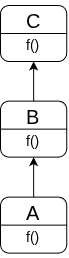
\includegraphics[width=0.06\textwidth]{images/SimpleDiagram.png}
  \caption{Simple graph}
  \label{fig:simpleDiagram}
\end{figure}

For the example above (Fig. \ref{fig:simpleDiagram}) a logical MRO could be $(A, B, C)$, this means that when the function f is executed from the class $A$ the implementation of $A$ will be prioritized over $B$, and the implementation of $B$ will be priorized over $C$.\\
However, the MRO of a class hierarchy is not always that straightforward, and conflicts can start to arise when we introduce multiple inheritance.
To demonstrate this, consider the following example, that represents a known problem called the diamond problem\cite{mondayezeStudiesObjectorientedProgramming2021}.
\begin{figure}[htbp]
  \centering
  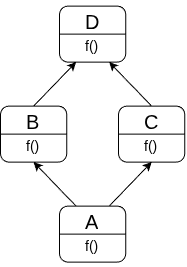
\includegraphics[width=0.15\textwidth]{images/DiamondProblem.png}
  \caption{Diamond problem graph}
  \label{fig:DiamondProblem}
\end{figure}

In this example (Fig. \ref{fig:DiamondProblem}), a conflict emerges when determining the MRO of class $A$, since $A$ inherits from both $B$ and $C$. This raises the question: Which implementation, $B$'s or $C$'s, does $A$ inherit from? 
This is where the C3 linearization algorithm comes into play, as it provides a consistent and predictable way to resolve this conflict, the algorithm says that we need to prioritize $B$ over $C$, because $B$ comes first in the class hierarchy, and therefore the MRO of $A$ will be $(A, B, C, D)$.

\subsection{C3 Linearization Algorithm}
\label{subsec:C3Linearization}
The C3 algorithm produces an MRO that is consistent with EPG, LPO, and monotonicity \cite{barrettMonotonicSuperclassLinearization1996} (all of these properties are formally defined in section \ref{subsec:PropertiesformalSpec}).

\subsubsection{EPG}
To understand the EPG, consider the following graph (Fig. \ref{fig:C3Diagram}). For this graph instead of ordering the classes from left to right,
 they are arranged by the weights of the directed edges, from smallest to largest.

\begin{figure}[htbp]
  \centering
  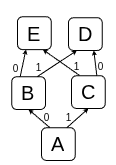
\includegraphics[width=0.15\textwidth]{images/NoneEPG.png}
  \caption{Inconsistent EPG}
  \label{fig:C3Diagram}
\end{figure}

This graph is inconsistent with the EPG, as the parent classes of $B$ and $C$ are ordered differently. A valid class hierarchy requires that for each class, the parent classes are ordered in the same way.
\subsubsection{LPO}
Consider the graph in Fig. \ref{fig:DiamondProblem}. An MRO that is consistent needs to respect the priority of the classes locally at each inheritance point; therefore, for this case, it cannot be $(A, C, B, D)$.
\subsubsection{Monotonicity}
If an MRO algorithm is consistency with monotonicity, it means that if a new class is added to the hierarchy the order of the previous MRO is preserved.

\subsection{Cameleer}
Cameleer is an automated tool for deductive verification in OCaml. It uses comments written in GOSPEL\cite{chargueraudGOSPELProvidingOCaml2019} (Generic OCaml Specification Language) to specify the properties of functions, and then leverages Why3 to verify these properties\cite{pereiraCameleerDeductiveVerification2021}.


\section{Formal Specification of C3 Linearization Algorithm}


\subsection{Ingredients}

Let \CC be a finite set of symbols, ranged over by \( C_0, C_1, \ldots, C_n \), possibly primed, which we refer to as \emph{classes}, and let \ordCC be an ordered set of classes. %\\

Consider $\mathcal P \subseteq \ordCC$ and $\DD \subseteq \CC \times \wp{(\mathcal P)}$.\\

The purpose of this document is to present the MRO algorithm,
which maps each $\CC$ with an ordered set of classes, $\mathcal P$. We show first the envisaged properties, then define it, and finally prove the definition ensures those properties.

\subsection{Properties}
\label{subsec:PropertiesformalSpec}


Let $D = \langle C, \{P_1, \dots, P_n\} \rangle \in \DD$, with $n\in\natz$.\\
Let $\mro(C) = \{C,C_1 \dots, C_m\}$, with $m \in \natz$.\\
\subsubsection{Consistency with the EPG} 
This property requires that
\(
\{P_1, \dots, P_n\} \subseteq \{C_1, \dots, C_m\}\,.
\)


\subsubsection{Consistency with the LPO}
For $m,n \geq 2$.
\begin{equation*}
\forall\,i,j\;\bigl(0\le i<j\le n \;\Longrightarrow \quad \exists\,p,q\;\bigl(0\le p<q\le m \wedge C_p=P_i \wedge C_q=P_j\bigr)\bigr)
\end{equation*}
\subsubsection{Consistency with monotonicity}

Let $D', D'' \in \DD$ \\
If $C \in \pi_2(D') \setminus \pi_2(D'')$, then\\ $\exists p,q. \ 0 < p < q \leq m \ \wedge \ C_p = C \ \wedge \ C_q = \pi_1(D'')$.

\subsection{Functions}

Let $\ordCC^*$ be a sequence of ordered sets of classes.\\
Let $L = (L_1, \ldots , L_n)$, $L \in \ordCC^*$\\
Let $C \in \mathcal{C}$\\

\subsubsection{Remove}

$\rem : \ordCC^* \times \CC \Rightarrow \ordCC^*$\\
\[
\rem(( \ ), C) = ( \ )
\]
\[
\rem(l::L, C) = l \setminus \{C\} :: \rem(L,C)
\]

\subsubsection{Merge}
$\mer : \ordCC^* \Rightarrow \ordCC $

\begin{equation*}
\mer(L)=
\begin{cases} 
\{C\} \cup \mer(\rem(L, C)), & \text{if (1), (2), (3)} \\
\text{fail}, & \text{otherwise}
\end{cases}
\end{equation*}

where:
\begin{align*}
&(1) \quad \exists k \in \oneToN, L_k \neq \emptyset \land C = \h(L_k) \\
&(2) \quad \forall j < k, C \neq \h(L_j) \\
&(3) \quad \forall i \in \oneToN, C \notin \texttt{tail}(L_i)
\end{align*}

\subsubsection{C3 Linearization}
$\cl: \DD \Rightarrow \ordCC$\\
$\text{Let } D = \langle C, P \rangle \text{ where } D \in \DD$\\
Let $D' = (D_1,D_2, \dots ,D_{|P|})$, such that \\
$\forall P_i \in P, \; \exists D_i \in \DD \text{ where } D_i = \langle P_i, P' \rangle$ where\\ $i \in  [\![1, |P|]\!]$.\\
Let $\texttt{C3linearization}$ be denoted as $\texttt{cl}$ for brevity.

\[
\texttt{cl}(D) =
\begin{cases}
\{C\} & \text{if } P = \emptyset \\
\{C\} \cup \mer\left( \left( \texttt{cl}(D_i) \right)_{D_i \in D'},\, P \right) & \text{otherwise}
\end{cases}
\]

\bibliographystyle{splncs04}
\bibliography{refs}

\end{document}
